%% Adaptado de 
%% http://www.ctan.org/tex-archive/macros/latex/contrib/IEEEtran/
%% Traduzido para o congresso de IC da USP
%%*****************************************************************************
% Não modificar

\documentclass[twoside,conference,a4paper]{IEEEtran}

%******************************************************************************
% Não modificar
\usepackage{IEEEtsup} % Definições complementares e modificações.

\usepackage[english,brazil]{babel}
\usepackage[utf8]{inputenc}

%% \usepackage{latexsym,amsfonts} % Disponibiliza fontes adicionais.

\usepackage[T1]{fontenc}
\usepackage{fbb}

\usepackage{animate}

\usepackage{theorem} 
%% \usepackage[cmex10]{amsmath} % Pacote matemático básico 
\usepackage{url} 
\usepackage{graphicx}
\usepackage{amsmath}
\usepackage{amssymb}
\usepackage{color}
\usepackage[pagebackref=true,breaklinks=true,colorlinks,bookmarks=false]{hyperref}
\usepackage[tight,footnotesize]{subfigure} 
\usepackage[noadjust]{cite} % Disponibiliza melhorias em citações.
%%*****************************************************************************

\begin{document}
\selectlanguage{brazil}
\renewcommand{\IEEEkeywordsname}{Palavras-chave}

%%*****************************************************************************

\urlstyle{tt}
% Indicar o nome do autor e o curso/nível (grad-mestrado-doutorado-especial)
\title{Algoritmos Genéticos + Redes Neurais = ?}
\author{%
 \IEEEauthorblockN{João Vitor Araki Gonçalves\,\IEEEauthorrefmark{1}}
 \IEEEauthorblockN{Lucy Miyuki Miyagusiku Narita\,\IEEEauthorrefmark{2}}
 \IEEEauthorblockA{Ciência da Computação - Graduação \\
                   \IEEEauthorrefmark{1}%
                   ra176353@students.ic.unicamp.br\\
                   \IEEEauthorrefmark{2}%
                   ra182851@students.ic.unicamp.br}
}

%%*****************************************************************************

\maketitle

%%*****************************************************************************
% Modifique as seções de acordo com o seu projeto

\section{Introdução}

Este trabalho tem como objetivo implementar e aplicar uma técnica de computação evolutiva na prática.
Algoritmos genéticos problemas são resolvidos através de um processo evolutivo que resulta na solução mais adequada dado algum critério, são, portanto, muito utilizados para problemas de otimização e de busca onde o crescimento exponencial das combinações faz de um algoritmo tradicional de busca inviável.

\section{Dependências}

O projeto foi desenvolvido em Python 3.X. As dependências se encontram no arquivo \texttt{requirements.txt}.

\section{Trabalho Proposto}

As redes neurais são o ponto central da revolução do \emph{Deep Learning}. A tecnologia avançou a ponto de ser capaz de sintetizar voz, reconhecer imagens e alterar o conteúdo de videos de forma a adulterar a informação passada originalmente.

Para este projeto, procuramos fazer o \emph{tunning} dos parâmetros de uma rede neural com um algoritmo genético. Trabalho que normalmente é feito "à mão" com base em experimentação e determinação destes valores de forma empírica.

O algoritmo foi implementado de forma genérica, sendo possível utilizá-lo com entradas genéricas, desde que sejam especificados as formas de \emph{crossover} e \emph{mutação} específicas para o problema que se deseja resolver.

\subsection{Indivíduo (Cromossomo)}

Nosso indivíduo é composto por 4 valores reais:

\begin{itemize}
    \item número de epochs
    \item quantidade de layers
    \item output space dimension para cada layer
    \item número de features
\end{itemize}

A função de \emph{fitness} foi dada pelo inverso da função de perda da rede.

\section{Resultados e Discussão}

\subsection{01}

\begin{itemize}
    \item rede: mnist
    \item tamanho da população: 10
    \item gerações (max): 100
    \item taxa de mutação:
    \item taxa de crossover:
    \item técnica de seleção: a melhor metade da população
    \item técnica de crossover: aleatóriamente seleciona um ou mais alelos para mutar, baseando-se na taxa de mutação dos alelos. Mutação de \emph{layers}: gera um número número aleatório e 
    \item técnica de mutação:
    \item epochs: [1-10]
    \item layers: [0-4]
    \item neurons: [100-2000]
    \item features: [1-4]
    \item critério de parada: limite de gerações atingido
    \item \textbf{melhor indivíduo}: Layers: 3, Neurons: [219  12 182], Loss: 0.06365562731241807, Epochs: 7
    \item loss: Figura \ref{fig:loss_mnist_01}
    \item accuracy: Figura \ref{fig:acc_mnist_01}
\end{itemize}

\begin{figure}[htbp]
        \centering 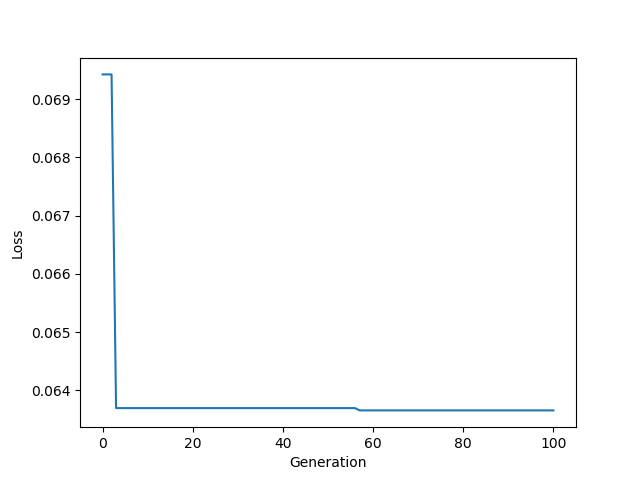
\includegraphics[width=1\columnwidth]{./imgs/01_mnist.png}
        \caption{
                \label{fig:loss_mnist_01}
                Loss
        }
\end{figure}
\begin{figure}[htbp]
        \centering 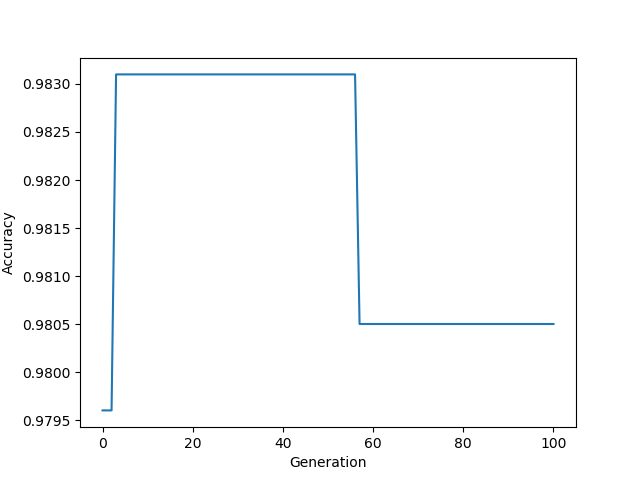
\includegraphics[width=1\columnwidth]{./imgs/01_mnist_acc.png}
        \caption{
                \label{fig:acc_mnist_01}
                Accuracy
        }
\end{figure}

\subsection{02}

\begin{itemize}
    \item rede: autoencoder (mnist)
    \item tamanho da população: 10
    \item gerações (max): 100
    \item taxa de mutação:
    \item taxa de crossover:
    \item técnica de seleção:
    \item técnica de crossover:
    \item técnica de mutação:
    \item epochs: [1-10]
    \item layers: [0-4]
    \item neurons: [100-2000]
    \item features: [1-4]
    \item critério de parada: limite de gerações atingido
    \item \textbf{melhor indivíduo}: Layers: 3, Neurons: [466 137 334], Loss: 0.060888413391448556, Epochs: 4
    \item loss: Figura \ref{fig:loss_mnist_auto_01}
    \item accuracy: Figura \ref{fig:acc_mnist_auto_01}
\end{itemize}

\begin{figure}[htbp]
        \centering 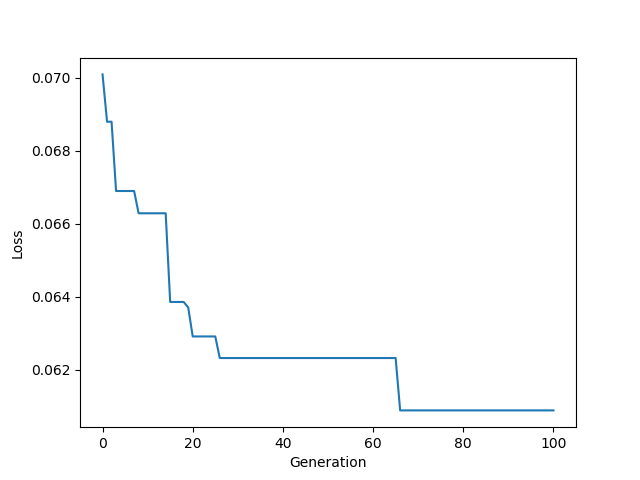
\includegraphics[width=1\columnwidth]{./imgs/01_mnist_auto.png}
        \caption{
                \label{fig:loss_mnist_auto_01}
                Loss
        }
\end{figure}
\begin{figure}[htbp]
        \centering 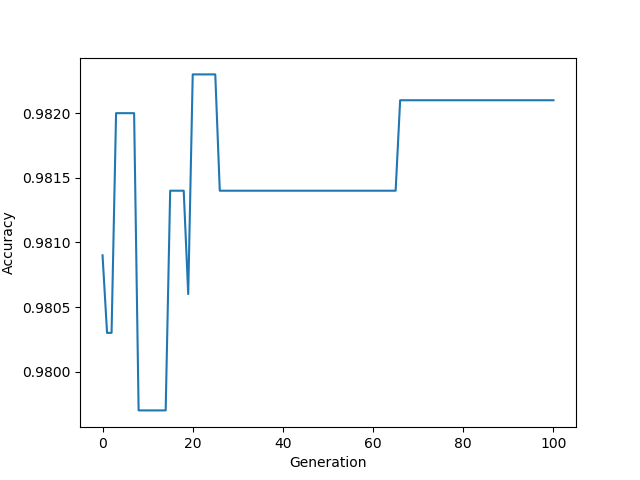
\includegraphics[width=1\columnwidth]{./imgs/01_mnist_auto_acc.png}
        \caption{
                \label{fig:acc_mnist_auto_01}
                Accuracy
        }
\end{figure}

\subsection{03}

\begin{itemize}
    \item rede: mnist (?)
    \item tamanho da população: 5
    \item gerações (max): 100
    \item taxa de mutação:
    \item taxa de crossover:
    \item técnica de seleção:
    \item técnica de crossover:
    \item técnica de mutação:
    \item epochs: [1-10]
    \item layers: [0-4]
    \item neurons: [100-2000]
    \item features: [1-4]
    \item critério de parada: limite de gerações atingido
    \item \textbf{melhor indivíduo}: Layers: 3, Neurons: [466 137 334], Loss: 0.060888413391448556, Epochs: 4
    \item loss: Figura \ref{fig:loss_mnist_auto_01}
    \item accuracy: Figura \ref{fig:acc_mnist_auto_01}
\end{itemize}

\begin{figure}[htbp]
        \centering 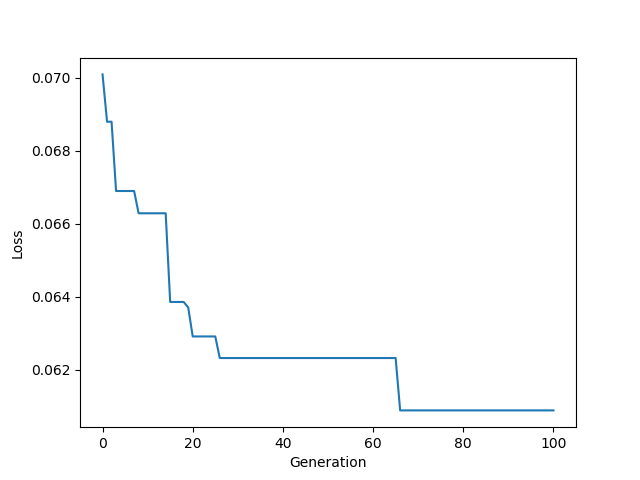
\includegraphics[width=1\columnwidth]{./imgs/01_mnist_auto.png}
        \caption{
                \label{fig:loss_mnist_auto_01}
                Loss
        }
\end{figure}
\begin{figure}[htbp]
        \centering 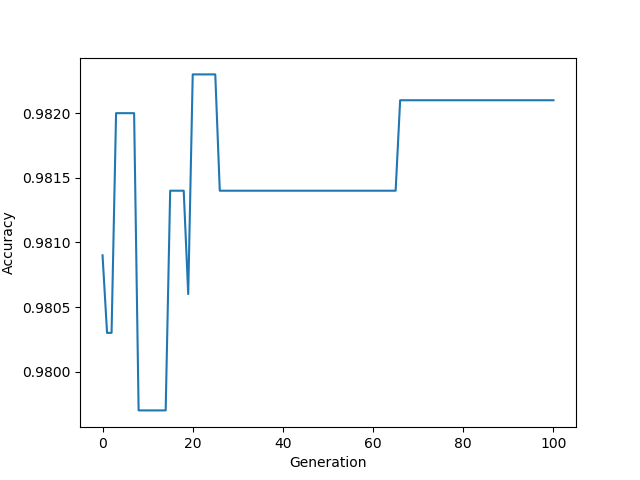
\includegraphics[width=1\columnwidth]{./imgs/01_mnist_auto_acc.png}
        \caption{
                \label{fig:acc_mnist_auto_01}
                Accuracy
        }
\end{figure}

\begin{itemize}
    \item tamanho da população
    \item critério de parada
    \item técnica de seleção
    \item técnica de crossover
    \item técnica de mutação
    \item método de substituição
    \item taxa de mutação
    \item taxa de crossover
\end{itemize}

\section{Conclusões}

Tivemos alguns problemas no decorrer do projeto por conta do tempo gasto como treinamento da rede para cada indivíduo gerado pelo algoritmo genético, além disso, alguns de nossos resultados (autoencoder de rostos) não foram tão bem sucedidos quanto esperado.

Ainda sim, gostaríamos de argumentar que o projeto pode ser considerado um sucesso no que se refere ao seu objetivo principal: implementar, aplicar e analisar os resultados obtidos através de um algoritmo genético aplicado a um problema real ou da literatura.


\cite{Rowling:1997}


%******************************************************************************
% Referências - Definidas no arquivo Relatorio.bib
 +----------------+

\bibliographystyle{IEEEtran}

\bibliography{Relatorio}


%******************************************************************************


\end{document}
